\documentclass{uwstat572}
\usepackage{amsmath}
\usepackage{color}
\usepackage{graphicx}

%%\setlength{\oddsidemargin}{0.25in}
%%\setlength{\textwidth}{6in}
%%\setlength{\topmargin}{0.5in}
%%\setlength{\textheight}{9in}

\renewcommand{\baselinestretch}{1.5} 


\bibliographystyle{plainnat}

\usepackage{color}
\usepackage{ulem}
\newcommand{\vmdel}[1]{\sout{#1}}
\newcommand{\vmadd}[1]{\textbf{\color{red}{#1}}}
\newcommand{\vmcomment}[1]{({\color{blue}{VM's comment:}} \textbf{\color{blue}{#1}})}

\begin{document}
%%\maketitle

\begin{center}
  {\LARGE Bayesian Lasso}\\\ \\
  {Annelise Wagner \\ 
    Department of Statistics, University of Washington Seattle, WA, 98195, USA
  }
\end{center}



\begin{abstract}
  The Bayesian Lasso, building on the interpretation of Tibshirani, places Laplace priors on linear regression coefficients to allow for Bayesian approaches to parameter and error estimation. An efficient Gibbs sampler allows for quick computation and may be exanded to other forms of penalized regression.
\end{abstract}

\section{Introduction}\label{Introduction}
Regression problems are an extremely common class of approaches to finding linear relationships (or more complex relationships) between a vector of $p$ explanatory variables, $x$, and a response variable $y$. \vmcomment{All vectors and matrices should be bolded.} 
The straight forward approach to these problems, even introduced at the most basic level of statistics, is ordinary least squares \vmadd{(OLS)} regression. 
\vmcomment{Maybe include some refs; also mention examples of scientific or engineering problems solved by regression.}

OLS regression is fairly well understood, allowing for estimates of regression coefficients, prediction, and error estimation. Despite this, ordinary least squares has a number of problems. Correlation between $x$ variables may conflate the relationship with $y$, resulting in biased estimates of regression coefficients \vmcomment{Reference?}.
Another problem that is becoming increasingly common with the prevalence of large datasets, a researcher may not know which of the $x$ variables are truly related to $y$, and may have $p$ explanatory variables when only $p'<p$ of them drive the relationship in $y$. While the relationship between some regressors and $y$ should be null, OLS will also tend to fit all regression coefficients with at least non-zero value, as this will usually produce minor decreases in the squared error \citep{seeger2008bayesian}.

This takes the problem of finding the best regression coefficients, and introduces a second problem of model selection. For small problems, a total of $2^p$ possible models exist and may be full explored and evaluated according to some information critirion such as AICC or BIC. For a problem like assessing DNA microarray data, where thousands or tens of thousands of data points are collected for tens or hundreds of people, individually assessing models becomes impossible \citep{ishwaran2005spike}.

This particular problem introduces two similar ideas, selection and shrinkage. \
\vmcomment{1) What particular problem?; 2) How can a problem introduce ideas?}
 A method is required that will either select which estimates will be non-zero, or an alternative view is that it needs to shrink estimates to zero. In the case of the gene expression data, a Bayesian approach akin to a constrained optimization problem known as spike and slab priors was used \cite{ishwaran2005spike}. 
 \vmcomment{Explain in words the gist of the idea behind spike and slab priors.}

Another form of penalized regression, the Least Absolute Shrinkage and Selection Operator (Lasso), limits the $L_1$ norm of coefficients to produce zero estimates for \vmadd{some of the} coefficients. 
This same idea can be found in signal processing, where Basis Pursuit seeks to select from many different waveforms by penalizing their $L_1$ norms \citep{chen2001atomic}.

One early shortcoming of the Lasso was a lack of estimation of variability. Simple solutions, such as bootstrap sampling, can easily be demonstrated to have problems overestimating zeros \citep{kyung2010penalized}.
\vmcomment{Do you mean ``overestimating the number of zero coefficients?}
In fact, it can be shown that these estimates are not even consistent as sample sizes increase \citep{shao1996bootstrap}. 
One approach based on a correction to sandwich estimation, point estimation of standard deviations \citep{fan2001variable}. 
\vmcomment{I didn't understand the last sentence --- please re-write.}

The Bayesian Lasso builds on the idea proposed by Tibshirani's Lasso, of treating the estimatimates as least squares estimates with Laplace prior distributions placed on regression parameters. 
By taking advantage of a \vmdel{reexpression} \vmadd{scale mixture of normals representation} of the Laplace distribution an effective Gibbs sampler can be created to produce credible intervals of \vmadd{regression coefficient} estimates \citep{tibshirani1996regression}.

\section{Background and Methods}
Linear regression assumes that we have some vector of responses, $\boldsymbol{y}$, which depend linearly on some covariates, $\boldsymbol{X}$. Formally, accounting for an error term, we wish to fit the model \[
\boldsymbol{y} = \mu \boldsymbol{1}_n + \boldsymbol{X}\boldsymbol{\beta}+\boldsymbol{\epsilon}\vmadd{,}
\] 
where $\boldsymbol{y}$ is an $n \times 1$ vector, $\mu$ is the mean of $\boldsymbol{y}$, $\boldsymbol{X}$ is a matrix of regressors (typically standardized), and $\boldsymbol{\epsilon}$ is a vector of indepedent and identically distributed zero mean normal variables with an unknown variance. For the sake of this discussion we will assume that the $\boldsymbol{y}$ has zero mean ($\mu=0$), noting that in practice this can be easily achieved by subtracting the sample mean estimate \vmadd{from $\mathbf{y}$}.

What is of interest is the regression coefficients, $\boldsymbol{\beta}$. These can be used for prediction when new values of regressors are given, or they may be of interest for their interpretation o\vmdel{n}\vmadd{f} the effects of certain regressor values on the dependent $\boldsymbol{y}$. Irrespective of the use, there are a number of approaches to finding the regressor coefficients. One familiar method, ordinary least squares, seeks to minimize least squares error\[
\min_{\boldsymbol{\beta}} \hspace{.1cm} (\boldsymbol{y}-\boldsymbol{X}\boldsymbol{\beta})^T(\boldsymbol{y}-\boldsymbol{X}\boldsymbol{\beta}).
\] While OLS estimates are a straight-forward and simple approach, Section~\ref{Introduction} details some of the shortcomings of this method.

Penalized regression takes a similar approach, trying to minimize the square error of predicted values, but with further constraints on regression coefficients. One form of penalization, known as bridge regression, takes the form  \[
\min_{\boldsymbol{\beta}}  \hspace{.1cm} (\boldsymbol{y}-\boldsymbol{X}\boldsymbol{\beta})^T(\boldsymbol{y}-\boldsymbol{X}\boldsymbol{\beta})+\lambda\sum_{j=1}^p|\beta_j|^q
\] for some $q\geq0$ \cite{park2008bayesian}. The cases where $q=1$ (Lasso Regression) and $q=2$ (Ridge Regression) have appealing and better understood properties. 
\vmcomment{Insert original, or as close to original as possible, references for ridge and bridge regression.}

The more desirous property of the Lasso is its ability to produce sparce estimates of parameters. It accomplishes this task by restricting solutions onto an $L_1$ 'ball' around the origin. This is more obvious from the dual formulation, 
\begin{align*}
\min_{\boldsymbol{\beta}}  \hspace{.1cm} &(\boldsymbol{y}-\boldsymbol{X}\boldsymbol{\beta})^T(\boldsymbol{y}-\boldsymbol{X}\boldsymbol{\beta})\\
\text{subject to} \hspace{.1cm}&\sum_{j=1}^p|\beta_j|\leq r
\end{align*}
for some $r$ determined by $\lambda$. Figure~\ref{LassoPlot} shows how this penalization compares to a Ridge Regression, Bridge Regression with $q=2$ which restricts solutions onto an $L_2$ ball \citep{park2008bayesian}.

\begin{figure}\label{LassoPlot}
  \centering
    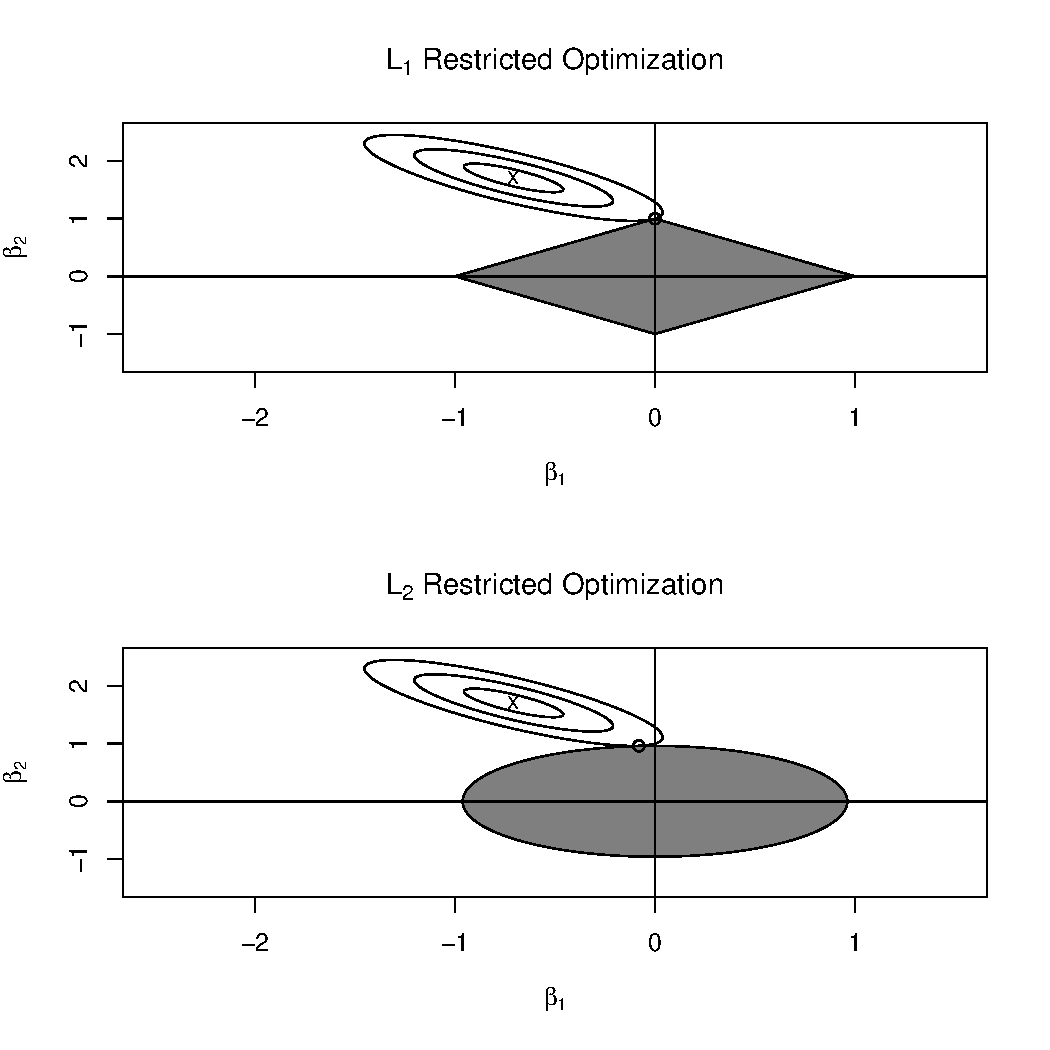
\includegraphics[width=0.7\textwidth]{LassoPlot.pdf}
  \caption{This example illustrates the tendancy for Lasso estimates to be driven to 0, compared with Ridge Regression estimates which are close to but not exactly 0 for $\beta_1$. \emph{\color{red} (I want to make this side by side, and 1:1)\color{black}} 
  \vmcomment{This picture needs explanation of what all the geometric objects mean in reference to the regression problem.}}
\end{figure}

For this reason we are most interested in the Lasso. The standard form representation, for some penalty weight $\lambda \geq 0$, has the form \[
\min_{\boldsymbol{\beta}}  \hspace{.1cm} (\boldsymbol{y}-\boldsymbol{X}\boldsymbol{\beta})^T(\boldsymbol{y}-\boldsymbol{X}\boldsymbol{\beta})+\lambda\sum_{j=1}^p|\beta_j|.
\] In the Lasso original derivation it was noted that these estimates can be equivalently viewed as posterior modes of OLS estimates, when independent Laplace priors are placed on the $\boldsymbol{\beta}$s \cite{tibshirani1996regression}.
\vmcomment{OLS estimates do not have posterior distributions, and no posterior modes too.}

The Bayesian Lasso, in keeping with Tibshirani's original interpretation, places independent Laplace (or double exponential) distributions on the parameters. 
Specifically, \vmadd{prior density}
\[
\pi(\beta|\sigma^2)=\prod_{j=1}^p\frac{\lambda}{2\sqrt{\sigma^2}}e^{-\lambda |\beta_j|/\sqrt{\sigma^2}}
\] 
is placed on each distribution, which results in a unimodal posterior. 
\vmcomment{Prior density cannot be placed on a distribution --- priors are placed on parameters; Also, what unimodal posterior are you talking about? Marginal posteriors of each regression coefficient? Is this known? 
If yes, provide a reference or a proof.}
Other prior distributions have been considered, but unimodality is key for Lasso estimates as non-unimodal posterior distributions cause convergence problems.
\vmcomment{Again, back up these claims; What unimodality are you talking about, prior or posterior?}

\subsection{Prior Distributions}
In keeping with our \vmdel{normal} errors being independent and identically distributed normals, then the response vector is distributed\vmdel{,} \vmadd{as follows}
\[
\mathbf{y}|\mu,\mathbf{X},\boldsymbol\beta,\sigma^2 \sim \mathcal{N}_n(\mu \mathbf{1}_n+\mathbf{X}\boldsymbol\beta,\sigma^2\mathbf{I}_n), \] but again noting that the vector $\mathbf{y}$ should be centered, resulting in $\mu=0$. Altneratively, an independent flat prior on $\mu$ can be used without affecting conjugacy of relevant variables.

The variance $\sigma^2$ can be given an inverse gamma prior distribution (while maintaining conjugacy), but the treatment by \cite{park2008bayesian} instead uses an improper prior, $1/\sigma^2$. This choice of $\sigma^2$ is also important in maintaining the unimodality of $\boldsymbol\beta$. 
\vmcomment{$\boldsymbol{\beta}$ cannot be unimodal, its distribution can be, but which one: prior or posterior?}

The variances of $\boldsymbol\beta$, $\tau_1^2,...,\tau_p^2$, are given independent distributions of the form, \[ \tau^2_j \sim \frac{\lambda^2}{2}e^{-\lambda^2\tau^2_j/2}d\tau^2_j.\] 
\vmcomment{Define prior for $\boldsymbol{\beta}$ first, then define priors for $\boldsymbol{\sigma}$ and $\boldsymbol{\tau}s$}

The regression parameters $\boldsymbol\beta$, conditioned on their variance estimates $\tau_1^2,...,\tau_p^2$, are given a normal prior, \[ 
\boldsymbol\beta|\sigma^2,\tau^2_1,...,\tau^2_p\sim\text{N}_p(\mathbf{0}_p,\sigma^2\mathbf{D}_\tau),\] with \[ \mathbf{D}_\tau=\text{diag}(\tau_1^2,...,\tau^2_p)\vmadd{,}
 \] 
which is not the double exponential prior intended. To arrive at the desired \vmdel{l}\vmadd{L}aplace distribution, the representation found in \citep{andrews1974scale} allows us to express the Laplace distribution as a scale mixture of normal distributions, \[ \frac{a}{2}e^{-a|z|}=\int^\infty_0
\frac{1}{\sqrt{2\pi s}}e^{-z^2/(2s)}\frac{a^2}{2}e^{-a^2s/2}ds.\] We can then integrate out $\tau^2_1,...,\tau^2_p$ to arrive at the desired distribution, \[ \pi(\boldsymbol\beta|\sigma^2)=\prod^p_{j=1}\frac{\lambda}{2\sqrt{\sigma^2}}e^{-\lambda|\beta_j|/\sqrt{\sigma^2}}, \] which is a Laplace prior. Again it is worth noting that conditioning on $\sigma^2$ produces a unimodal distribution, while independent Laplace priors on $\boldsymbol\beta$ causes convergence problems.
\vmcomment{Again, I am not getting this. Conditional on $\sigma$, $\beta$s are independently distributed. What convergence problems do you have in mind, under what MCMC sampling strategy?}

\subsection{Full Conditionals}
With our priors properly defined, we are then able to sample consecutively from the full conditional distributions of $\boldsymbol\beta$, $\sigma^2$, and $\tau^2_1,...,\tau^2_p$. First defining the matrix $\mathbf{A}=\mathbf{X}^T\mathbf{X}+\mathbf{D}_\tau^{-1}$ for simplification, \[
\boldsymbol\beta|\mathbf{y},\mathbf{X},\sigma^2,\boldsymbol\tau^2 \sim \text{N}_p(\mathbf{A}^{-1}\mathbf{X}^T\mathbf{y},\sigma^2\mathbf{A}^{-1}) \]. The full conditional of the variance is, \[ \sigma^2|\mathbf{y},\mathbf{X},\boldsymbol\beta,\boldsymbol\tau^2 \sim \text{InvGamma}\left(\alpha'=\frac{n-1}{2}+\frac{p}{2},\beta'=(\mathbf{y}-\mathbf{X}\boldsymbol\beta)^T(\mathbf{y}-\mathbf{X}\boldsymbol\beta)+\frac{\boldsymbol\beta\mathbf{D}_\tau^{-1}\boldsymbol\beta}{2}\right). \] And lastly the full conditionals of the coefficient variances $\tau^2_1,...,\tau^2_p$ are independent, with \[
\frac{1}{\tau_j^2} | \boldsymbol\beta, \sigma^2, \lambda \sim \text{InvGaussian}\left(\mu'=\sqrt\frac{\lambda^2\sigma^2}{\beta_j^2}, \lambda'=\lambda^2\right). \] We can then produce a Gibbs sampler by consecutively sampling each of these distributions.

\subsection{Empirical Bayesian Selection of $\lambda$}
One point that has yet to be addressed is the selection of the hyperparameter $\lambda$.
 A typical approach such as cross-validation is suitable for many applications, but the Bayesian approach taken \vmdel{in} \vmadd{by} \cite{park2008bayesian} allows us to take advantage of the Monte Carlo EM algorithm proposed \vmdel{in} \vmadd{by} \cite{casella2001empirical}. 
 Here, we start with $\lambda^{(0)}$ based on the ordinary least squares estiamtes 
 \[ 
\lambda^{(0)}=\frac{p\sqrt{\hat\sigma^2_{LS}}}{\Sigma^p_{j=1}|\hat\beta_j^{LS}|}\vmadd{,} 
\] 
which is then updated after a run of the Gibbs sampler according to \[ 
\lambda^{(k)}=\sqrt\frac{2p}{\Sigma^p_{j=1}E_\lambda[\tau^2_j|\mathbf{y}]}
\] by replacting the explectation with an average from the Gibbs sample. 

\vmcomment{I did not understand this Monte Carlo EM at all. Where are the missing data and complete data likelihood? What is $k$ indexing? Needs a detailed explanation.} 


\emph{Note: I feel like I'm mimicing the original paper too much in some places, but I also feel like there's not really a lot of nuance in how a lot of this is explained. Any tips?}

\vmadd{I would expand on some of the derivations. For example, you probably should show how integration of $\tau$s leads to a Laplace distribution. Also, derivation of full conditionals could be helpful, at least some of them.}

\section{Results}

\section{Discussion}

\bibliography{stat572}

\end{document}









